\documentclass[11pt,a4paper]{article}
\usepackage[T1]{fontenc}
\usepackage[utf8]{inputenc}
\usepackage{lmodern}
\usepackage{microtype}
\usepackage[margin=2.2cm]{geometry}
\usepackage{booktabs}
\usepackage{graphicx}
\usepackage{float}
\usepackage{amssymb}
\usepackage{xcolor}
\usepackage{enumitem}
\usepackage{caption}
\usepackage{titlesec}
\usepackage{array}
\newcolumntype{L}[1]{>{\raggedright\arraybackslash}p{#1}}
\usepackage[colorlinks=true,linkcolor=black,urlcolor=blue!50!black]{hyperref}

\definecolor{title}{HTML}{1F3A5F}
\titleformat{\section}{\Large\bfseries\color{title}}{\thesection.}{0.5em}{}
\titleformat{\subsection}{\large\bfseries\color{title}}{}{0em}{}
\setlist{nosep,leftmargin=1.4em}
\setlength{\parindent}{0pt}
\setlength{\parskip}{5pt}
\captionsetup{font=small,labelfont=bf}
\graphicspath{{../figures/}}

\begin{document}

\begin{center}
{\LARGE\bfseries\color{title} Phish or Not?}\\[6pt]
{\large Does a phishing e-mail detector still work on e-mail sources it has never seen?}\\[14pt]
\textit{Week 2 report: data, learning plan, baseline, state of the art}\\[4pt]
Imene KHELIL, Florian GALLOT, Ambroise RÉCOPÉ de TILLY-BLARU, Dylan HUANG\\[2pt]
{\small ESILV, Machine Learning 2026, OCC, November 2026}
\end{center}

\section*{Summary}
\begin{itemize}
\item \textbf{Data:} 82,486 e-mails from six public corpora. 13\% are exact or near-duplicates; we remove them (71,386 left).
\item \textbf{Main problem found:} the source corpus can be guessed from the text 98.7\% of the time, so a model can learn ``which corpus is this?'' instead of ``is this phishing?''.
\item \textbf{Baseline:} TF-IDF + logistic regression. On a normal test set: F1 = 0.991, false-positive rate (FPR) = 0.84\%.
\item \textbf{On a source it has never seen:} F1 drops to 0.79--0.93 and the FPR rises to 5.6--24\%. Only 58\% of modern phishing (Nazario, 2015--2022) is caught.
\item \textbf{AutoML v0.1:} picks a more complex model that is slightly better on the normal test set but worse on all 4 unseen sources. Next step: select models on unseen sources, not on a random split.
\end{itemize}

%-----------------------------------------------------------------
\section{Business scope and problem}
Most attacks on companies start with an e-mail (stolen passwords, malware, fake invoices). A spam/phishing filter is only useful if it keeps working on e-mails from other companies, campaigns or years than the ones it was trained on. The two errors do not cost the same: a missed phishing e-mail can compromise an account, and a legitimate e-mail sent to quarantine costs time and trust. Because malicious mail is a small share of real traffic, even a few percent of false positives can drown the real alerts.

\textbf{Task.} Each e-mail is a text (subject + body) with a label: 1 = spam/phishing, 0 = legitimate. The model outputs the probability of class 1 and we predict 1 above 0.5. We also know the source corpus of each e-mail, but we only use it to build the evaluation splits, never as a feature (a real filter would not have it).

\textbf{Metrics.} Precision, recall and F1 on the malicious class; false-positive rate FPR = FP / (FP + TN), our main safety metric; ROC-AUC; Brier score for calibration. Our data is 48\% malicious, much more than real traffic, so we also give Prec@5\%: the precision the same model would have if only 5\% of e-mails were malicious.

%-----------------------------------------------------------------
\section{Dataset}
We use the Phishing Email Dataset from Kaggle (N.\,A.~Alam, co-author of Al-Subaiey et al.\ 2024; licence CC BY-SA 4.0), downloaded with \texttt{kagglehub}; the SHA-256 of each file is checked (\texttt{data/README.md}). Counts match the published totals: 82,486 e-mails, 42,891 malicious, 39,595 legitimate. We use the six per-source files and not the merged CSV, because the merged file has no source column and its text was already pre-processed.

\begin{table}[H]\centering\small
\caption{The six corpora, before and after removing duplicates.}
\setlength{\tabcolsep}{4pt}
\begin{tabular}{lL{5cm}lrr}
\toprule
Corpus & What it is & Period & E-mails (raw $\rightarrow$ kept) & \% malicious \\
\midrule
CEAS\_08 & CEAS 2008 spam-filter challenge & 2008 & 39,154 $\rightarrow$ 31,781 & 49.3 \\
Enron & Enron employees' mailboxes + spam & $\sim$2000--2002 & 29,767 $\rightarrow$ 27,719 & 45.9 \\
Ling & Linguist mailing list + spam & $<$ 2001 & 2,859 $\rightarrow$ 2,742 & 15.5 \\
Nazario & Phishing mailbox (monkey.org), CC BY 4.0 & 2015--2022 & 1,565 $\rightarrow$ 1,435 & 100 \\
Nigerian\_Fraud & 419 scam collection, CC BY-SA 3.0 & 1998--2007 & 3,332 $\rightarrow$ 2,637 & 100 \\
SpamAssassin & Apache SpamAssassin public corpus & 2002 & 5,809 $\rightarrow$ 5,072 & 20.5 \\
\midrule
\textbf{Total} & & & \textbf{82,486 $\rightarrow$ 71,386} & \textbf{47.5} \\
\bottomrule
\end{tabular}
\end{table}

\textbf{Why did we choose this dataset?} This is the largest public dataset with real e-mails from several independent sources and a source label, and it is the one used by the papers we compare with. Its limits: label 1 is mostly ordinary spam (only Nazario and Nigerian\_Fraud are targeted fraud), most e-mails are from 2000--2008, and two corpora have no legitimate e-mail at all. We use it for academic work only, do not redistribute the raw files, and only show aggregate statistics and single words in this report.

%-----------------------------------------------------------------
\section{Data exploration and quality}
\begin{figure}[H]\centering
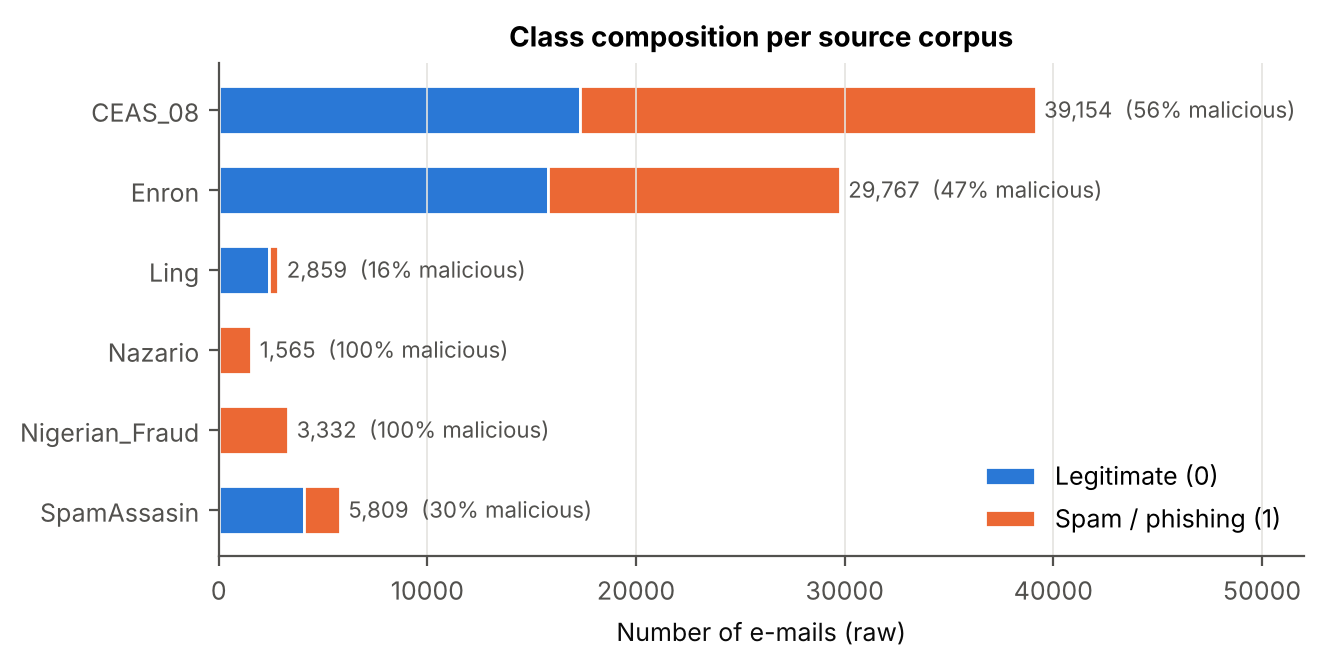
\includegraphics[width=.75\linewidth]{fig1_composition.png}
\caption{Class mix per source. Two corpora contain only malicious e-mails.}
\end{figure}

\begin{itemize}
\item \textbf{Missing values:} Enron and Ling have no sender, receiver, date or URL field at all. Any metadata feature would reveal the corpus, so we only use subject + body (missing subjects, 0--2\%, become empty strings).
\item \textbf{Duplicates:} 988 exact copies and 13,314 near-duplicates (MinHash-LSH, Jaccard $\ge$ 0.8) in 3,203 groups. The four biggest groups (3,919 e-mails) are one fake ``CNN Alerts'' malware campaign from August 2008. We keep one e-mail per group, before any split.
\item \textbf{Length:} from a few characters to 4.6 million (base64 attachments in Nazario). We cut every e-mail at 20,000 characters ($<$ 1.1\% affected per source). Length is not a stable signal: spam is shorter than ham in CEAS\_08 but longer in SpamAssassin.
\item \textbf{Class balance:} 47.5\% malicious overall, so no re-sampling. Imbalance is inside sources (Ling 15.5\%, SpamAssassin 20.5\%, Nazario and Nigerian 100\%), so the split is stratified by source and label.
\item \textbf{Form:} Enron and Ling were distributed lower-cased and tokenised (``file : hplno 530 . xls''); the other corpora are raw text. Years range from 2002 to 2022.
\end{itemize}

\subsection{Can a model cheat by recognising the corpus?}
We trained a classifier to predict the source (not the label) from the text:
\begin{table}[H]\centering\small
\caption{Accuracy of predicting the source corpus (6 classes).}
\begin{tabular}{lr}
\toprule
Input & Accuracy \\
\midrule
Raw text & 98.7\% \\
Lower-case, no punctuation & 96.1\% \\
Same + URLs, e-mails and digits masked & 95.0\% \\
5 style statistics only (length, case\ldots) & 85.5\% \\
Chance (most frequent source) & 44.5\% \\
\bottomrule
\end{tabular}
\end{table}
Even after cleaning, the corpus is recognised 95\% of the time, and the source alone (without any text) already gives 58.2\% label accuracy. The giveaway words are names (\texttt{vince}, \texttt{kaminski}), host names (\texttt{monkey}), mailing-list topics (\texttt{opensuse}, \texttt{linguistics}) and anonymisation leftovers (\texttt{zzzzteana}): nothing to do with phishing. This is the shortcut our leave-one-source-out test is designed to expose.

\subsection{Pre-processing}
\begin{itemize}
\item Text = subject + body, cut at 20,000 characters.
\item Remove exact and near-duplicates before the split.
\item Lower-case, drop punctuation and underscores (so raw and tokenised corpora look the same).
\item Optional: replace URLs, e-mail addresses and digits by tokens (years and phone codes identify corpora). Some Enron addresses still escape this mask; the fix is planned for v0.2 (AI\_AUDIT \#9).
\item No case or punctuation features, no re-sampling.
\end{itemize}

%-----------------------------------------------------------------
\section{Learning and testing plan}
\begin{itemize}
\item \textbf{Hold-out test (20\%):} 14,278 e-mails, stratified by source $\times$ label, saved in \nolinkurl{data/processed/split.csv} and used once at the end. Two asserts check that no duplicate group and no identical text is on both sides.
\item \textbf{Model selection:} stratified $k$-fold cross-validation on the training part only (5 folds for the baseline, 3 for AutoML).
\item \textbf{Leave-one-source-out (LOSO):} train on five sources, test on the sixth. Nazario and Nigerian\_Fraud have no legitimate e-mail, so only recall is reported for them.
\item \textbf{No leakage:} TF-IDF, scaler and feature selection are inside a scikit-learn \texttt{Pipeline}, refitted in every fold; the source is never a feature.
\item \textbf{Over/under-fitting:} train vs validation F1 for every model.
\end{itemize}
We also checked whether near-duplicates crossing the split inflate the score: F1 0.9907 with a random split vs 0.9909 with duplicates kept together, so the effect is negligible here.

%-----------------------------------------------------------------
\section{Baseline}
\textbf{Model.} TF-IDF on single words (100k features) + L2 logistic regression. It is the standard text baseline, its coefficients can be read, and it is the model of our main reference (Bhuiyan \& Bhuiyan 2026).

\textbf{Choosing $C$.} Training F1 reaches 1.000 for $C \ge 100$ (the model memorises), while validation F1 is flat from $C = 10$. We use the one-standard-error rule and keep the most regularised $C$ within one standard error of the best: $C = 100$. The curve is so flat that another computer picked $C = 30$, for a validation F1 lower by only 0.0002. Probabilities are well calibrated (Brier score 0.007).

\begin{figure}[H]\centering
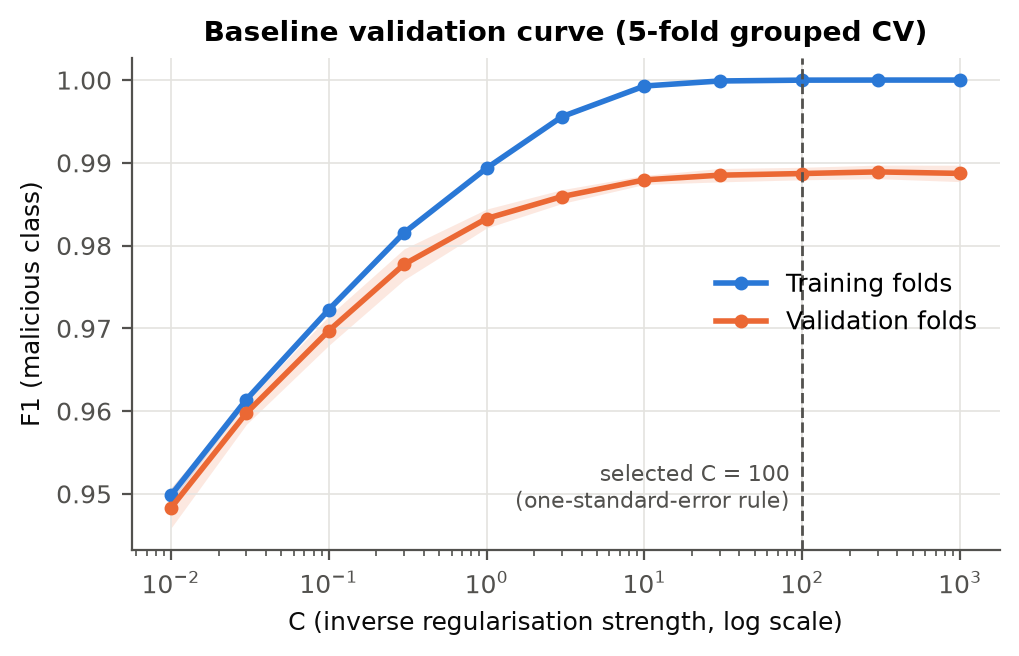
\includegraphics[width=.6\linewidth]{fig5_validation_curve.png}
\caption{Validation curve of the baseline (5 folds).}
\end{figure}

\textbf{What it learned.} Good signals appear among the top words (\texttt{remove}, \texttt{kindly}, \texttt{viagra}, \texttt{urgent}, \texttt{bank}), but also shortcuts: years (\texttt{2004}, \texttt{2008}), people and hosts (\texttt{enron}, \texttt{vince}, \texttt{kaminski}, \texttt{monkey}) and \texttt{713}, the Houston phone code. They do not hurt the normal test score; they show up on unseen sources.

\begin{table}[H]\centering\small
\caption{Baseline on the normal test set and on each unseen source, next to Bhuiyan \& Bhuiyan (2026).}
\setlength{\tabcolsep}{5pt}
\begin{tabular}{lrrrrrr}
\toprule
Test on & Recall & F1 & FPR & Prec@5\% & Ref.\ F1 & Ref.\ FPR \\
\midrule
\textbf{Normal hold-out} & \textbf{0.992} & \textbf{0.991} & \textbf{0.8\%} & \textbf{0.861} & -- & -- \\
Unseen: CEAS\_08 & 0.984 & 0.934 & 11.9\% & 0.302 & 0.899 & 11.4\% \\
Unseen: Enron & 0.910 & 0.830 & 24.0\% & 0.167 & 0.820 & 22.7\% \\
Unseen: Ling & 0.908 & 0.820 & 5.6\% & 0.460 & 0.837 & 5.1\% \\
Unseen: SpamAssassin & 0.973 & 0.795 & 12.3\% & 0.294 & 0.843 & 12.7\% \\
Unseen: Nazario & 0.581 & -- & -- & -- & -- & -- \\
Unseen: Nigerian\_Fraud & 0.992 & -- & -- & -- & -- & -- \\
\bottomrule
\end{tabular}
\end{table}

\begin{figure}[H]\centering
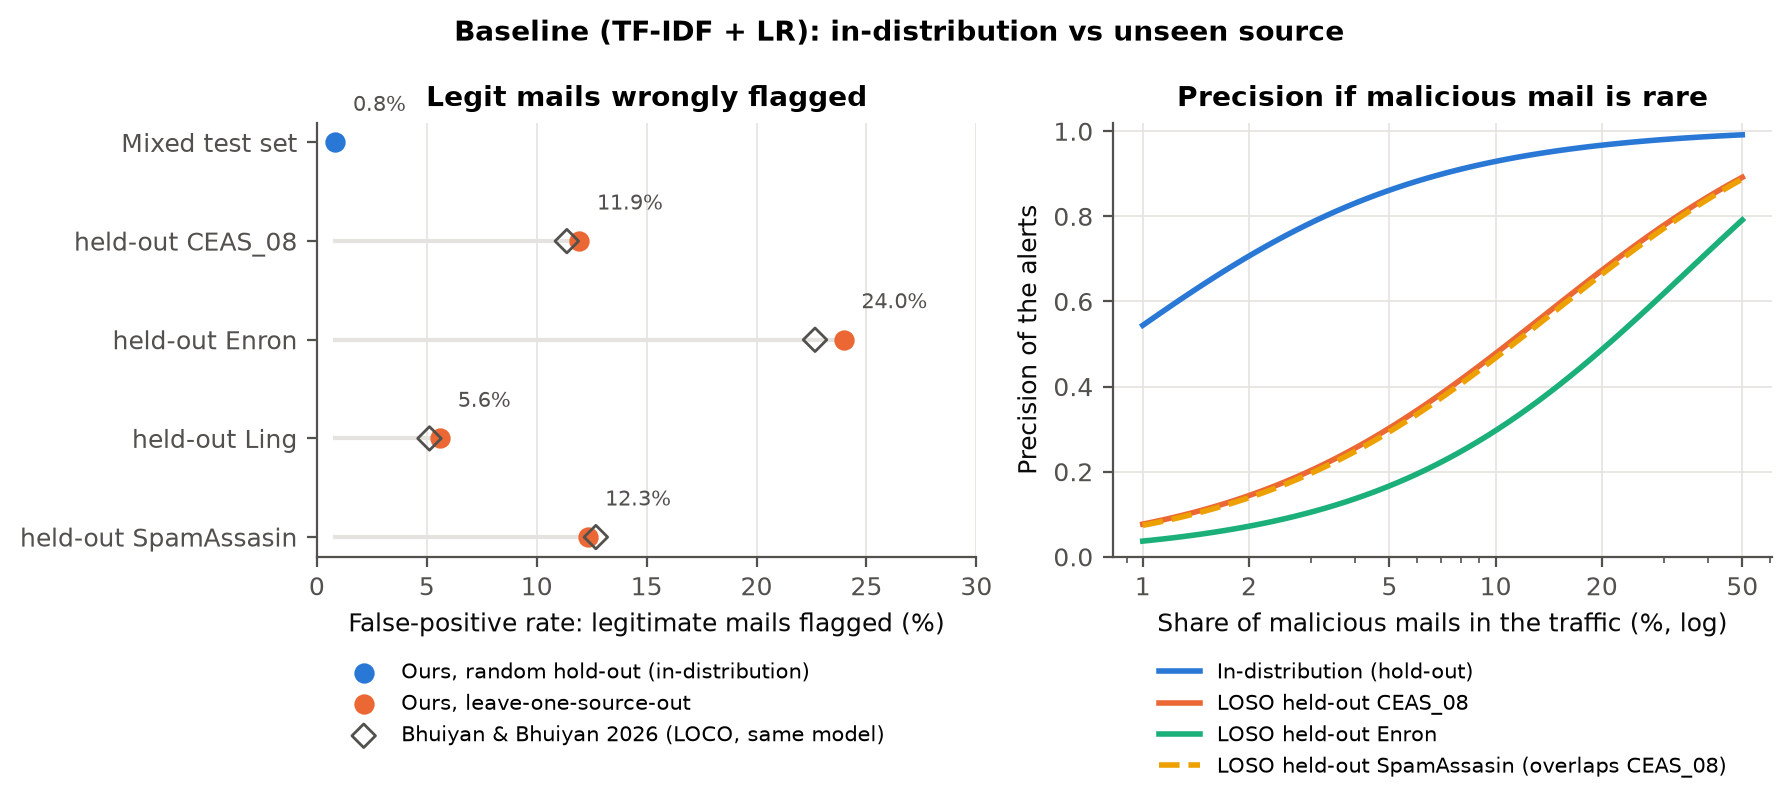
\includegraphics[width=.95\linewidth]{fig7_generalisation_gap.png}
\caption{Left: FPR on the normal test vs on an unseen source. Right: share of real alerts depending on how much of the traffic is malicious.}
\end{figure}

\textbf{Results.} On an unseen source, F1 drops from 0.991 to 0.79--0.93 and the FPR is 7 to 29 times higher. If 5\% of the traffic were malicious, fewer than one alert in three would be real on CEAS\_08, Enron or SpamAssassin. Only 58\% of modern phishing (Nazario) is caught, against 99\% of the older Nigerian scams. This is not caused by our cleaning dropping non-ASCII characters (that effect is 0.3 points). Our numbers match the published ones within 0.05 F1 and 1.3 FPR points, which supports our protocol.

%-----------------------------------------------------------------
\section{State of the art}
\begin{table}[H]\centering\small
\caption{Published results on this dataset.}
\begin{tabular}{L{3.5cm}L{3.2cm}L{3.5cm}L{4.4cm}}
\toprule
Reference & Model & Protocol & Result \\
\midrule
Al-Subaiey et al.\ 2024 (dataset authors) & TF-IDF + linear SVM & Random 80/20 split & F1 0.99 \\
Ahmed \& Pourmoafi 2026 & TF-IDF + LR; DistilBERT & Random split + adversarial set & F1 0.986 / 0.991; $-$35 pts accuracy under attack \\
Bhuiyan \& Bhuiyan 2026 & TF-IDF + LR / SVM & Leave-one-corpus-out & F1 0.82--0.90; source guessed 97.2\% \\
\midrule
\textbf{Ours (baseline)} & \textbf{TF-IDF + LR} & \textbf{Dedup + frozen split + LOSO} & \textbf{F1 0.991; unseen 0.79--0.93; Nazario 0.58} \\
\bottomrule
\end{tabular}
\end{table}
On a random split, every paper reaches about 99\%: the score is saturated. The leave-one-corpus-out result is the relevant benchmark for our question. None of these papers removes duplicates.

%-----------------------------------------------------------------
\section{AutoML pipeline}
\textbf{Pipeline.} Each configuration is one scikit-learn pipeline: cleaning (minimal or masked) $\rightarrow$ features (word TF-IDF, optional character 3--5-grams, optional 8 hand-made statistics such as length, number of URLs, urgency words) $\rightarrow$ optional $\chi^2$ selection $\rightarrow$ model (logistic regression, linear SVM, complement naive Bayes, SGD, ridge classifier, decision tree). Optuna (TPE sampler, median pruning) tunes it on 20,000 training e-mails with 3-fold CV and mean F1 as the objective.

\textbf{What happened.} The first run let the SVM go up to $C = 1000$ with no time limit; it did not converge and some trials took over 200\,s, so we stopped it (AI\_AUDIT \#6). The second run capped $C$ at 100 with a 25-minute budget; we stopped it after 34 trials (23 completed, 11 pruned). We recovered the parameters by replaying the seeded sampler and re-checked the top three scores (0.9827). The best is a ridge classifier (trial 25) on masked text with word 1--2-grams and character 3--5-grams (150k features, $\alpha = 0.044$).

Five of six families are within 0.005 CV F1 of each other; only the decision tree is far behind (0.89).

\begin{table}[H]\centering\small
\caption{Baseline vs AutoML, same test set and same unseen sources.}
\begin{tabular}{lrrrr}
\toprule
Test on & Baseline F1 & AutoML F1 & Baseline FPR & AutoML FPR \\
\midrule
\textbf{Normal hold-out} & \textbf{0.991} & \textbf{0.990} & \textbf{0.84\%} & \textbf{0.68\%} \\
Unseen: CEAS\_08 & 0.934 & 0.920 & 11.9\% & 10.6\% \\
Unseen: Enron & 0.830 & 0.803 & 24.0\% & 19.1\% \\
Unseen: Ling & 0.820 & 0.728 & 5.6\% & 8.5\% \\
Unseen: SpamAssassin & 0.795 & 0.746 & 12.3\% & 14.7\% \\
Nazario recall & 0.58 & 0.62 & -- & -- \\
\bottomrule
\end{tabular}
\end{table}

\begin{figure}[H]\centering
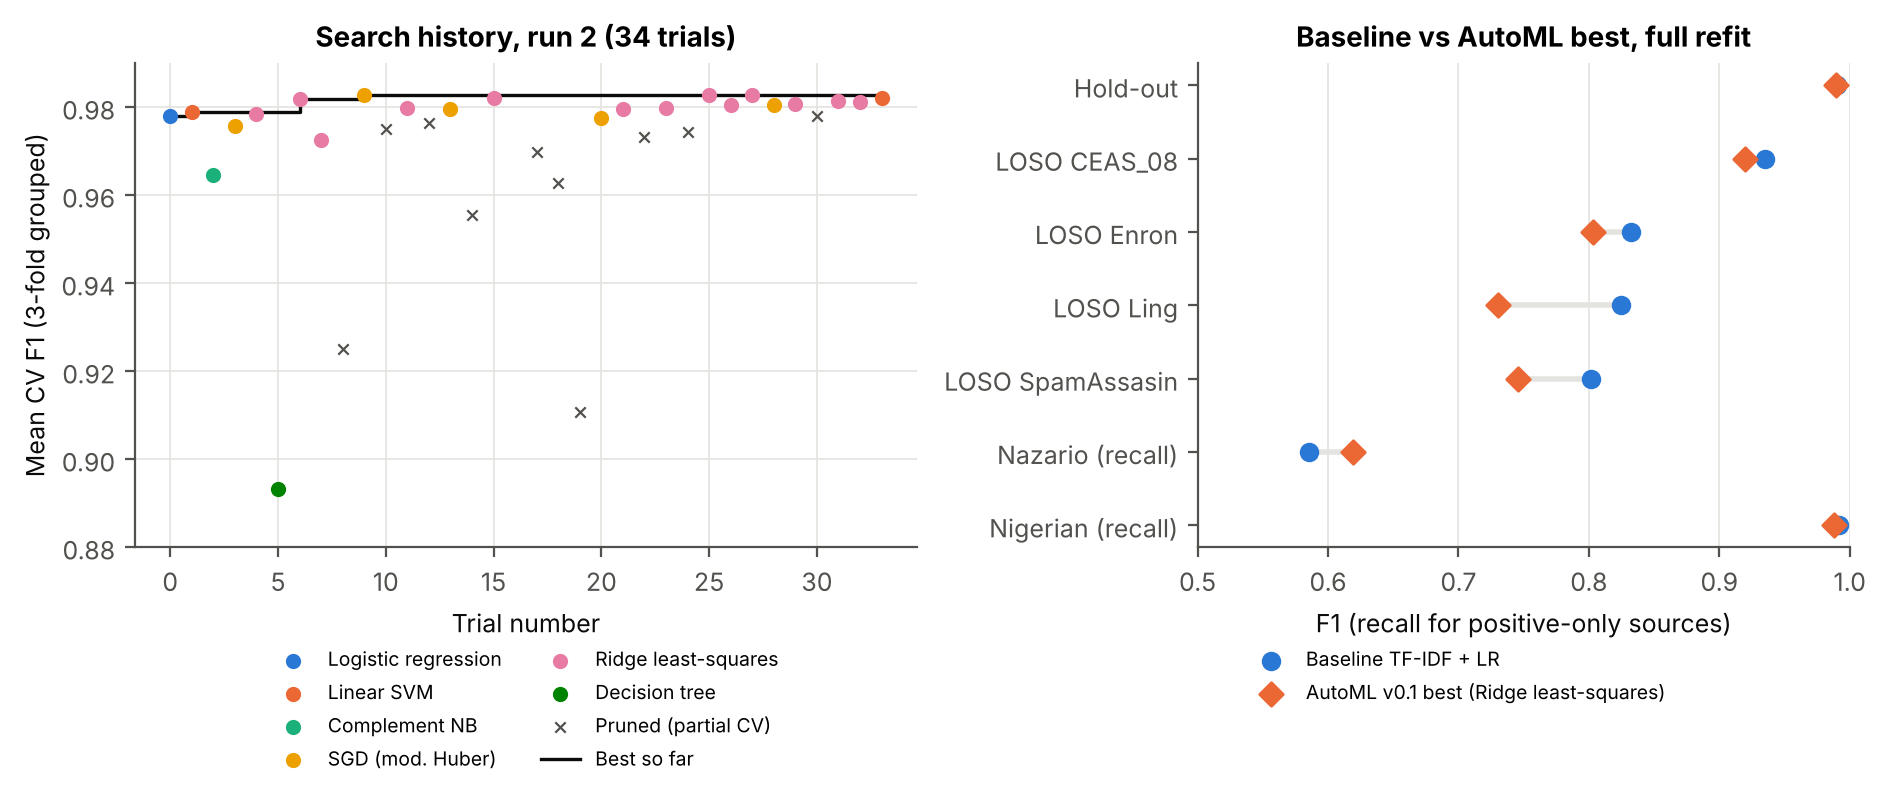
\includegraphics[width=\linewidth]{fig8_automl.png}
\caption{Left: search history. Right: baseline vs AutoML on each test.}
\end{figure}

\begin{itemize}
\item \textbf{Normal test:} AutoML has fewer false positives but misses more malicious e-mails (lower recall).
\item \textbf{Unseen sources:} AutoML has a lower F1 on all 4 sources. Only Nazario recall goes up.
\item \textbf{Why:} the chosen model is more complex (training F1 = 1.000). It fits the training corpora better, artefacts included, and transfers worse. Optimising a random-split score rewards memorising the corpora: the selection criterion is the problem, not the model family.
\end{itemize}

%-----------------------------------------------------------------
\section{Uncertainty, risks and plan}
\textbf{Confidence intervals.} We resampled the 14,278 test e-mails 2,000 times (bootstrap) to get 95\% intervals, and compared the two models on the same resamples (paired test).

\begin{table}[H]\centering\small
\caption{Normal test set: estimate [95\% bootstrap interval].}
\begin{tabular}{llll}
\toprule
 & Recall & F1 & FPR \\
\midrule
Baseline & 0.992 [0.990, 0.994] & 0.991 [0.990, 0.993] & 0.84\% [0.64, 1.06] \\
AutoML v0.1 & 0.987 [0.984, 0.989] & 0.990 [0.988, 0.991] & 0.68\% [0.51, 0.87] \\
\midrule
\textbf{Difference (AutoML $-$ baseline)} & \textbf{$-$0.005, $p<0.001$} & \textbf{$-$0.002, $p=0.04$} & \textbf{$-$0.16 pts, $p=0.17$} \\
\bottomrule
\end{tabular}
\end{table}
The recall loss of AutoML is significant, the F1 loss is borderline, and the lower FPR could be noise. On unseen sources the 95\% (Wilson) intervals are narrow, e.g.\ Enron FPR 24.0\% [23.3, 24.7], because each source has thousands of e-mails; the real uncertainty is the spread between sources, and we only have four binary sources to measure it.

\subsection{Risks}
\begin{itemize}
\item \textbf{Shortcuts:} the model uses names, years, hosts and formatting. We track them with the top words and the source-prediction test.
\item \textbf{Selection leakage:} hyper-parameters are chosen with all sources, including the one later left out. For the baseline we measured it: re-choosing $C$ without that source changes LOSO F1 by at most 0.005. It may be larger for AutoML, which searches much more.
\item \textbf{Labels:} label 1 is mostly spam, so conclusions about phishing rely on Nazario.
\item \textbf{Time:} most training data is from 2000--2008; modern phishing is under-detected.
\item \textbf{Threshold:} 0.5 is not a good operating point when the share of malicious mail changes.
\end{itemize}

\subsection{Plan for the next versions}
\begin{enumerate}
\item \textbf{Select on unseen sources:} choose hyper-parameters with an inner leave-one-source-out, and save every trial so a stopped search loses nothing.
\item \textbf{Remove artefacts:} fix the masking of Enron addresses (10.7\% of Enron e-mails still contain \texttt{hou}/\texttt{ect}; a prototype brings it to 0.4\%), then block names, hosts and years.
\item \textbf{Operating point:} pick the threshold for FPR $\le$ 1\% and report recall at that threshold.
\item \textbf{Ensembles:} voting or stacking of the best linear models.
\item \textbf{Model outside the course:} fine-tuned DistilBERT: does it rely less on corpus artefacts?
\item \textbf{Fresh test set:} a few recent, anonymised phishing e-mails from our own inboxes.
\end{enumerate}

%-----------------------------------------------------------------
\section*{AI usage}
We used Claude (Anthropic) as allowed by the course policy: for code, EDA drafts, literature search and wording. The important prompts are in \texttt{ai\_governance/PROMPT\_LOG.md}. \texttt{ai\_governance/AI\_AUDIT.md} lists twelve errors we found in AI-generated code and text and how we fixed them (for example a masking regex that created a new corpus artefact, an invalid evaluation plan, a hyper-parameter chosen at the edge of the grid, and report numbers that no longer matched the results). Every number in this report comes from \texttt{run\_all.sh}, which runs the whole project with \texttt{bash}; the tables were copied from its output files (\texttt{reports/latex/tables}).

\section*{References}
{\small
\begin{enumerate}
\item I.~Bhuiyan, T.~Bhuiyan. The fragility of phishing detection models: evidence from cross-corpus transfer, prevalence shift, artifact learning, and evasion risk. \emph{Big Data and Cognitive Computing} 10(7):211, 2026.
\item A.~Al-Subaiey et al. Novel interpretable and robust web-based AI platform for phishing email detection. \emph{Computers and Electrical Engineering}, 2024. arXiv:2405.11619.
\item T.~Ahmed, S.~Pourmoafi. Adversarial robustness of phishing email detection: TF-IDF + logistic regression vs fine-tuned DistilBERT. arXiv:2607.18429, 2026.
\item A.\,I.~Champa, M.\,F.~Rabbi, M.\,F.~Zibran. Phishing Email Curated Datasets. Zenodo 8339691 (CC BY 4.0).
\item A.\,Z.~Broder. On the resemblance and containment of documents. IEEE SEQUENCES, 1997.
\item R.~Geirhos et al. Shortcut learning in deep neural networks. \emph{Nature Machine Intelligence} 2:665--673, 2020.
\item S.~Kapoor, A.~Narayanan. Leakage and the reproducibility crisis in ML-based science. \emph{Patterns} 4(9), 2023.
\item T.~Hastie, R.~Tibshirani, J.~Friedman. \emph{The Elements of Statistical Learning}, 2nd ed., Springer, 2009.
\item T.~Akiba et al. Optuna: a next-generation hyperparameter optimization framework. KDD, 2019.
\item SANS Internet Storm Center. ``CNN -- My Custom Alert'', diary 4841, 8 August 2008.
\end{enumerate}
}
\end{document}
